\documentclass[11pt,a4paper,oneside,openright]{book}
\usepackage[spanish,activeacute,es-noshorthands]{babel}
\usepackage[utf8]{inputenc}
\usepackage[T1]{fontenc}
\usepackage{lmodern}
\usepackage{amsmath, amssymb, amsthm}
\usepackage{graphicx}
\graphicspath{{figuras/m15/}{figuras/}}
\usepackage[dvipsnames]{xcolor}
\usepackage{listings}
\usepackage{geometry}
\geometry{margin=2.5cm, headheight=14pt}
\usepackage{microtype}
\usepackage{booktabs}
\usepackage{longtable}
\usepackage{enumitem}
\usepackage{fancyhdr}
\usepackage{tcolorbox}
\tcbuselibrary{skins, breakable}
\usepackage{caption}
\captionsetup{font=small, labelfont=bf}
\usepackage{hyperref}
\hypersetup{
  colorlinks=true, linkcolor=NavyBlue, citecolor=ForestGreen, urlcolor=BrickRed,
  pdftitle={M15 --- Topologia de redes en CubeSats},
  pdfauthor={INTISAT --- Documentacion tecnica}
}

\definecolor{cbox-intui}{HTML}{2C5282}
\definecolor{cbox-intui-bg}{HTML}{EBF8FF}
\definecolor{cbox-warn}{HTML}{C53030}
\definecolor{cbox-warn-bg}{HTML}{FFF5F5}
\definecolor{cbox-ok}{HTML}{2F855A}
\definecolor{cbox-ok-bg}{HTML}{F0FFF4}
\definecolor{cbox-tech}{HTML}{B7791F}
\definecolor{cbox-tech-bg}{HTML}{FFFBEB}
\definecolor{cbox-payload}{HTML}{6B46C1}
\definecolor{cbox-payload-bg}{HTML}{FAF5FF}

\newtcolorbox{intui}{
  colback=cbox-intui-bg, colframe=cbox-intui, sharp corners=northwest,
  arc=2pt, boxrule=1pt, fonttitle=\bfseries, title=Intuicion, breakable
}
\newtcolorbox{cuidado}{
  colback=cbox-warn-bg, colframe=cbox-warn, sharp corners=northwest,
  arc=2pt, boxrule=1pt, fonttitle=\bfseries, title=Cuidado, breakable
}
\newtcolorbox{logrado}{
  colback=cbox-ok-bg, colframe=cbox-ok, sharp corners=northwest,
  arc=2pt, boxrule=1pt, fonttitle=\bfseries, title=Para INTISAT, breakable
}
\newtcolorbox{tecnico}{
  colback=cbox-tech-bg, colframe=cbox-tech, sharp corners=northwest,
  arc=2pt, boxrule=1pt, fonttitle=\bfseries, title=Detalle tecnico, breakable
}
\newtcolorbox{payloadbox}{
  colback=cbox-payload-bg, colframe=cbox-payload, sharp corners=northwest,
  arc=2pt, boxrule=1pt, fonttitle=\bfseries, title=Referencias, breakable
}

\definecolor{codebg}{HTML}{F8F9FA}
\lstdefinestyle{c}{
  basicstyle=\ttfamily\footnotesize,
  backgroundcolor=\color{codebg},
  keywordstyle=\color{NavyBlue}\bfseries,
  commentstyle=\color{ForestGreen}\itshape,
  stringstyle=\color{BrickRed},
  numbers=left, numberstyle=\tiny\color{gray},
  frame=single, framerule=0.4pt, rulecolor=\color{gray},
  breaklines=true, captionpos=b, language=C,
  showstringspaces=false, tabsize=2,
}
\lstdefinestyle{py}{
  basicstyle=\ttfamily\footnotesize,
  backgroundcolor=\color{codebg},
  keywordstyle=\color{NavyBlue}\bfseries,
  commentstyle=\color{ForestGreen}\itshape,
  stringstyle=\color{BrickRed},
  numbers=left, numberstyle=\tiny\color{gray},
  frame=single, framerule=0.4pt, rulecolor=\color{gray},
  breaklines=true, captionpos=b, language=Python,
  showstringspaces=false, tabsize=2,
}

\pagestyle{fancy}
\fancyhf{}
\renewcommand{\headrulewidth}{0.4pt}
\fancyhead[L]{\small M15 --- Topologia de redes en CubeSats}
\fancyhead[R]{\small \leftmark}
\fancyfoot[C]{\thepage}
\renewcommand{\chaptermark}[1]{\markboth{#1}{}}

\title{\Huge\bfseries M15 --- Topologia de redes\\[0.3em]
  \LARGE en CubeSats\\[0.5em]
  \large Como se conectan los subsistemas y como se ejerce el control\\
  \normalsize De I2C a CSP, de estrella a pub/sub. 6 misiones analizadas + propuesta INTISAT}
\author{Equipo INTISAT}
\date{Mayo 2026}

\begin{document}

\frontmatter
\maketitle

\chapter*{Prefacio}

Este manual responde a una pregunta que no se hace explicitamente
en las reuniones pero que define todo lo demas: \textbf{cuando dos
subsistemas del CubeSat quieren hablarse, $\zeta$como lo hacen?}

La respuesta tiene dos capas:

\begin{enumerate}[leftmargin=2em]
  \item \textbf{Capa fisica}: el bus electrico --- I2C, SPI, CAN, RS-485.
    Cables, voltajes, baudrates, terminadores.
  \item \textbf{Capa logica}: el protocolo encima del bus --- comandos,
    framing, direcciones, errores, retries. Aqui aparecen CSP, CANopen,
    Software Bus de cFS, ports de F\textquotesingle{}.
\end{enumerate}

\textbf{Por que importa.} En el manual M12 (maquinas de estado)
estudiamos \emph{como cada subsistema decide que hacer}. En el M13
estudiamos \emph{como otros lo hicieron}. Pero entre la decision
y la accion hay una capa intermedia: \textbf{como viajan los
comandos por el satelite}. Esa capa es la \emph{topologia de red}.

\textbf{Que vamos a sacar de aca.}

\begin{enumerate}[leftmargin=2em]
  \item Un vocabulario claro: capas OSI adaptadas a CubeSats.
  \item Los 5-6 buses fisicos que veras en cualquier mision.
  \item Las 5 topologias clasicas (estrella, bus, anillo, malla,
    pub/sub) y donde aparecen.
  \item La eleccion concreta de 6 misiones de referencia (FloripaSat,
    OreSat, AAUSAT, UPSat, NASA cFS, NASA F\textquotesingle{}), con su diagrama.
  \item Una matriz comparativa.
  \item Una propuesta concreta para INTISAT, con direcciones I2C,
    velocidades y protocolo de aplicacion.
\end{enumerate}

\textbf{Como leerlo.} Capitulos 1--3 son el marco conceptual. Capitulos
4--9 son una mision cada uno (independientes, podes saltar al que te
interesa). Capitulo 10 es la matriz. Capitulo 11 cierra con la
recomendacion para INTISAT.

\tableofcontents

\mainmatter

% ============================================================================
\chapter{Topologia, bus y control: tres ideas distintas}
% ============================================================================

\section{La trampa de mezclar las tres palabras}

En las reuniones se mezclan tres conceptos que son ortogonales:

\begin{itemize}[leftmargin=2em]
  \item \textbf{Bus fisico:} el medio electrico. I2C, SPI, CAN, RS-485,
    UART. Es \emph{hardware}.
  \item \textbf{Topologia:} la \emph{forma} de las conexiones. Estrella,
    bus multidrop, anillo, malla, distribuida.
  \item \textbf{Control:} \emph{quien decide que hace cada subsistema}.
    Centralizado (OBC manda), distribuido (cada uno autonomo),
    pub/sub (eventos sin jefe), compile-time (la topologia se fija al
    compilar).
\end{itemize}

\begin{intui}
La misma topologia puede ejercer control distinto. Por ejemplo:
\emph{estrella} se puede operar como ``el OBC manda todo'' (FloripaSat)
o como ``el OBC coordina pero cada perif. tiene su FSM'' (AAUSAT).
\emph{Mismo cableado, control distinto.}
\end{intui}

\section{Las capas (modelo OSI adaptado)}

El modelo OSI clasico tiene 7 capas. En un CubeSat, casi siempre
implementas 3 o 4 de ellas:

\begin{figure}[h]
  \centering
  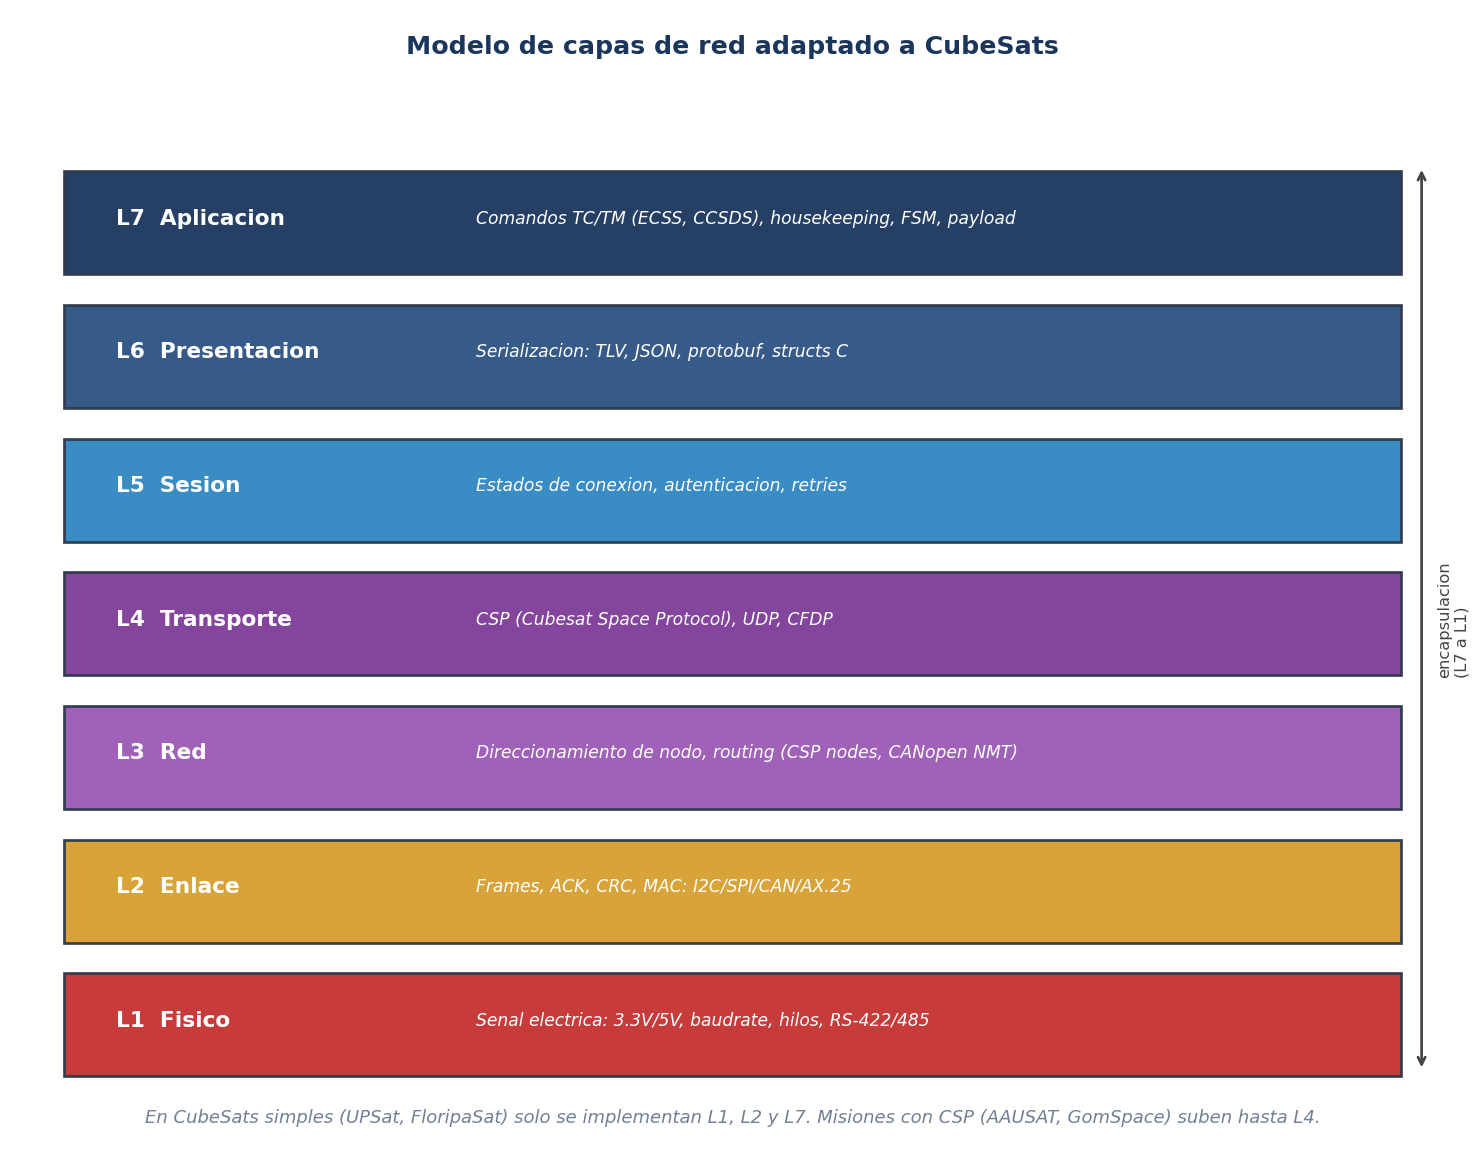
\includegraphics[width=0.92\textwidth]{fig01_capas_osi.png}
  \caption{Modelo de capas adaptado a CubeSats. CubeSats simples
  (UPSat, FloripaSat) implementan L1, L2 y L7 directamente. Misiones
  con CSP suben hasta L4.}
  \label{fig:m15-capas}
\end{figure}

\textbf{Para cada capa, una decision concreta:}

\begin{itemize}[leftmargin=2em]
  \item \textbf{L1 (fisico)}: voltaje, baudrate, hilos.
  \item \textbf{L2 (enlace)}: formato de frames, CRC, ACK.
  \item \textbf{L3 (red)}: direcciones de nodo, routing.
  \item \textbf{L4 (transporte)}: confiabilidad, retries, fragmentacion.
  \item \textbf{L7 (aplicacion)}: telecomandos, telemetria,
    file-transfer.
\end{itemize}

\section{Que pasa si solo implementas L1 y L7 (UPSat style)}

Es lo mas comun en CubeSats 1U sencillos. Tenes I2C como L1, mandas
bytes directos como L7 y no hay capas intermedias. \textbf{Funciona},
pero pierdes:

\begin{itemize}[leftmargin=2em]
  \item \textbf{Retransmision automatica} si una lectura falla.
  \item \textbf{Direccionamiento logico} (todo es ``escribi en
    direccion I2C 0x20'', no ``mandale comando GET\_TLM al EPS'').
  \item \textbf{Portabilidad}: si manana cambias I2C por CAN, hay que
    reescribir todo el codigo de aplicacion.
\end{itemize}

A cambio gana simplicidad. Para una mision de 6 meses sin
re-trabajo, suele alcanzar.

% ============================================================================
\chapter{Buses fisicos disponibles}
% ============================================================================

Antes de hablar de topologias, hace falta entender que opciones
electricas existen.

\begin{figure}[h]
  \centering
  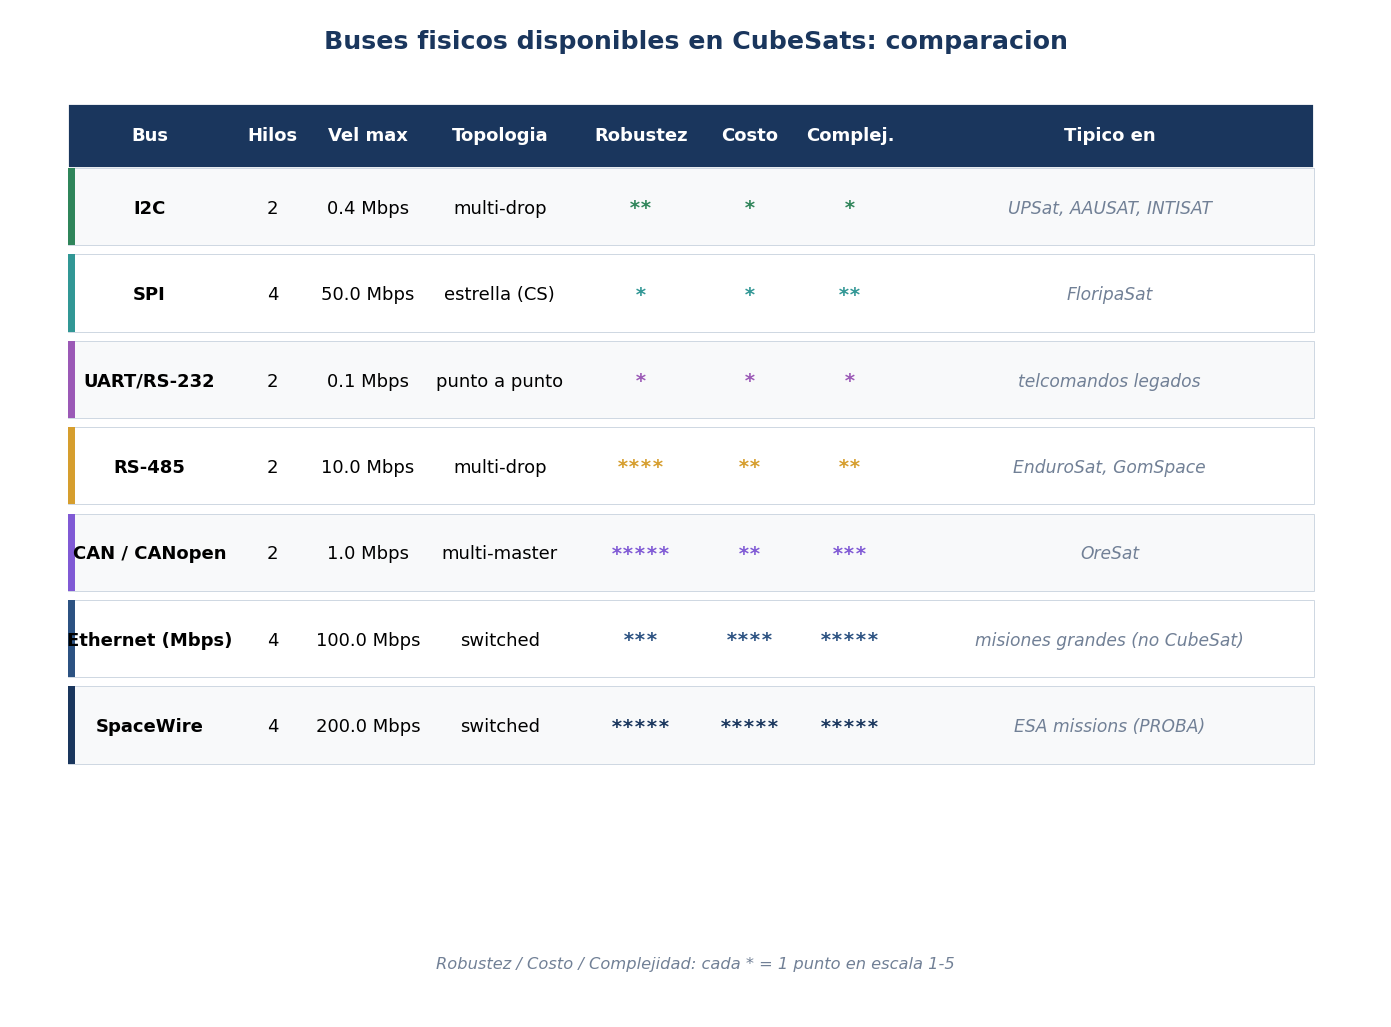
\includegraphics[width=\textwidth]{fig02_buses_comparados.png}
  \caption{Buses fisicos tipicos en CubeSats. La columna ``Tipico
  en'' indica donde aparece cada bus de verdad.}
  \label{fig:m15-buses}
\end{figure}

\section{I2C}

\textbf{2 hilos} (SDA + SCL), open-drain con pull-ups, half-duplex,
hasta 400 kHz tipico (1 MHz Fast-mode+ con cuidado).

\begin{itemize}[leftmargin=2em]
  \item \textbf{Pro:} simplisimo. Casi todo MCU lo tiene.
    Direccionamiento de 7 bits, hasta 127 esclavos teoricos.
  \item \textbf{Contra:} susceptible a glitches (pull-ups marginales,
    longitud de cable). No hay deteccion de error nativa --- si una
    lectura llega corrompida, no te enteras a menos que agregues CRC
    a nivel de aplicacion.
\end{itemize}

\textbf{Usado en:} UPSat, AAUSAT, INTISAT (target), GomSpace (modulos
chicos), EnduroSat (algunos modulos).

\section{SPI}

\textbf{4 hilos} (SCLK + MOSI + MISO + CS por esclavo), full-duplex,
hasta 50 MHz teorico (1-10 MHz tipico en CubeSat).

\begin{itemize}[leftmargin=2em]
  \item \textbf{Pro:} muy rapido. Ideal para sensores de alta tasa
    (camaras, ADCs).
  \item \textbf{Contra:} necesitas una linea CS por cada esclavo. Si
    queres 5 esclavos, son 5 GPIOs adicionales. No hay direccionamiento
    --- el CS \emph{es} la direccion.
\end{itemize}

\textbf{Usado en:} FloripaSat (bus principal), interfaces SD,
sensores rapidos como IMUs.

\section{CAN / CANopen}

\textbf{2 hilos diferenciales} (CAN\_H + CAN\_L), hasta 1 Mbps en
CubeSat (5 Mbps en CAN-FD), multi-master con arbitraje por ID.

\begin{itemize}[leftmargin=2em]
  \item \textbf{Pro:} robusto electricamente. Broadcast nativo. Multi-master:
    cualquier nodo puede iniciar transmision. Arbitraje no-destructivo:
    en colision gana el ID mas bajo sin perder mensaje.
  \item \textbf{Contra:} requiere transceiver fisico (chip TJA1042 o
    similar) en cada nodo. Stack de software mas grande que I2C.
\end{itemize}

\textbf{CANopen} agrega encima un perfil de aplicacion estandar (CiA
301): Object Dictionary, NMT (Network Management), SDOs y PDOs.

\textbf{Usado en:} OreSat (todo el satelite), industria automotriz
(de donde sale), GomSpace en sus modulos mas modernos.

\section{RS-485}

\textbf{2 hilos diferenciales}, half-duplex, hasta 10 Mbps a 12 m, o
100 kbps a 1.2 km. Lo mas viejo y mas robusto de la lista.

\begin{itemize}[leftmargin=2em]
  \item \textbf{Pro:} inmune a ruido por ser diferencial. Multi-drop
    sin transceivers complejos.
  \item \textbf{Contra:} half-duplex, sin direccionamiento nativo (lo
    agregas tu).
\end{itemize}

\textbf{Usado en:} algunos EPS comerciales (Spacemanic, EnduroSat),
interfaces con instrumentos cientificos.

\section{SpaceWire}

\textbf{4 pares diferenciales}, hasta 200+ Mbps. El bus profesional de
ESA y NASA para misiones medianas y grandes.

\begin{itemize}[leftmargin=2em]
  \item \textbf{Pro:} rapidisimo, switched, ECC. Estandar formal
    ECSS-E-ST-50-12C.
  \item \textbf{Contra:} sobre-ingeniado para un 1U. Hardware caro
    (FPGA dedicado).
\end{itemize}

\textbf{Usado en:} PROBA-1/2/3 (ESA), Mars Reconnaissance Orbiter,
JUICE. \textbf{No es para CubeSats chicos.}

\section{UART / RS-232 punto a punto}

\textbf{2 hilos} (TX + RX), velocidad libre (9600--921600 baudios
tipico), solo entre 2 dispositivos.

\begin{itemize}[leftmargin=2em]
  \item \textbf{Pro:} 100\% simple. Es lo que usa cualquier radio
    UHF como interfaz al OBC.
  \item \textbf{Contra:} solo dos puntos. No es un bus, es un cable.
\end{itemize}

\textbf{Usado en:} interfaz radio-OBC en casi todos los CubeSats,
debugging, conexion a PC.

% ============================================================================
\chapter{Las 5 topologias clasicas}
% ============================================================================

\begin{figure}[h]
  \centering
  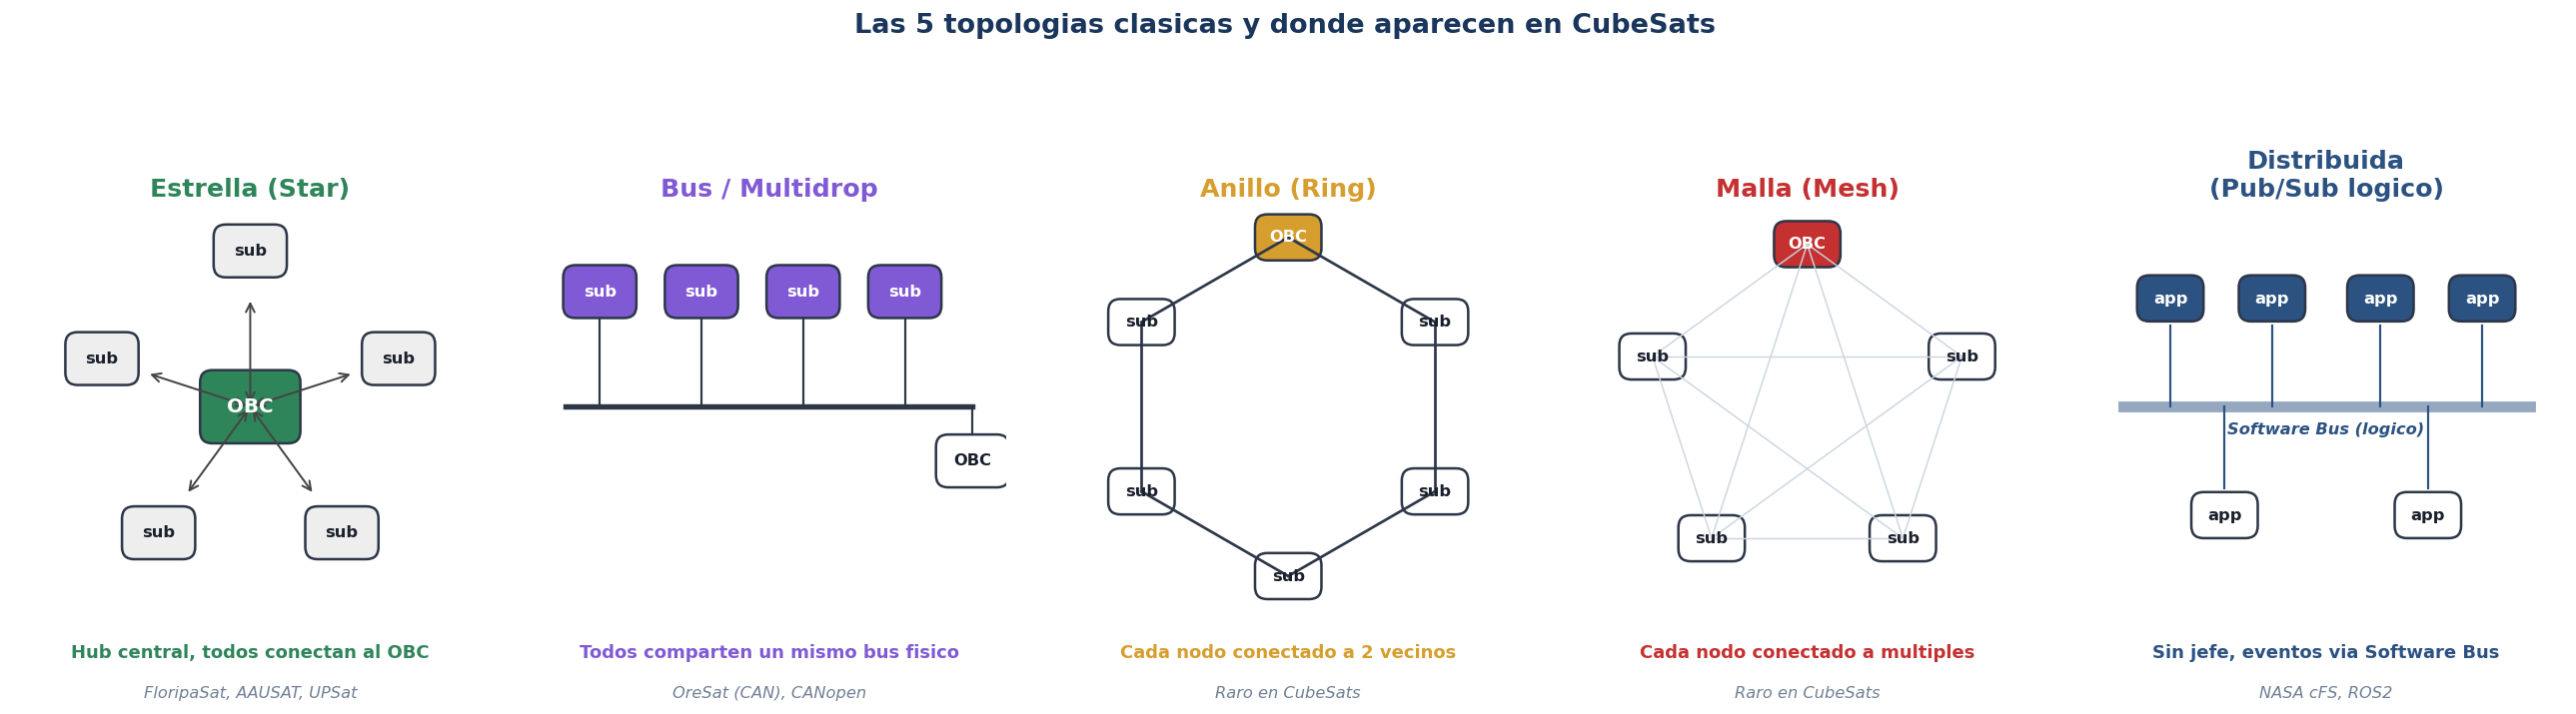
\includegraphics[width=\textwidth]{fig03_topologias_clasicas.png}
  \caption{Las 5 topologias clasicas y donde aparecen en CubeSats
  reales. La distribuida \emph{pub/sub} es logica, no fisica.}
  \label{fig:m15-topo}
\end{figure}

\section{Estrella (Star)}

Un nodo central (el OBC) y N perifericos conectados radialmente al
centro. \textbf{Es la topologia mas comun en CubeSats}.

\textbf{Ventajas:}
\begin{itemize}[leftmargin=2em]
  \item Simple de razonar: ``todos hablan con el OBC''.
  \item Facil de debuggear: si X no responde, miras el cable de X.
  \item Aislamiento de falla parcial: si EPS falla, el ADCS todavia
    habla con el OBC.
\end{itemize}

\textbf{Desventajas:}
\begin{itemize}[leftmargin=2em]
  \item El OBC es punto unico de fallo. Si se cuelga, nadie habla
    con nadie.
  \item Si el bus fisico es compartido (I2C), un periferico mal hecho
    puede colgar el bus para todos.
\end{itemize}

\section{Bus / Multidrop}

Todos los subsistemas comparten un mismo cable fisico (un par
diferencial en CAN, dos hilos en I2C). Cualquiera puede enviar; el
protocolo decide quien gana.

\textbf{Ventajas:}
\begin{itemize}[leftmargin=2em]
  \item Cableado minimo: 2-3 hilos para todo el satelite.
  \item Hot swap real (en CAN): podes desconectar un nodo y el bus
    sigue.
  \item Broadcast nativo: 1 mensaje llega a todos.
\end{itemize}

\textbf{Desventajas:}
\begin{itemize}[leftmargin=2em]
  \item Mas complejo de debuggear (todos hablan al mismo cable).
  \item Necesitas un protocolo de arbitraje (CAN lo trae built-in,
    I2C no).
\end{itemize}

\section{Anillo (Ring)}

Cada nodo conectado a 2 vecinos. Mensajes circulan hasta llegar al
destinatario.

\textbf{Donde aparece:} casi nunca en CubeSats. Mas comun en redes
LAN viejas (Token Ring) y en algunas misiones grandes (FireWire
networks). Lo nombramos por completitud.

\section{Malla (Mesh)}

Cada nodo conectado a varios. Multiples caminos hasta cualquier destino.

\textbf{Donde aparece:} raro en CubeSats. Mas comun en redes
inalambricas (Zigbee, Thread). Util cuando la tolerancia a fallos
es critica y el costo de cableado no importa.

\section{Distribuida / Pub-Sub logico}

\textbf{No es una topologia fisica, es logica.} El bus puede ser
cualquier cosa (I2C, CAN, memoria compartida, ROS topics). La idea
es: \textbf{nadie es el jefe}. Hay un \emph{Software Bus} al que las
aplicaciones publican mensajes y otras se suscriben. Quien publica no
sabe quien escucha.

\textbf{Ventajas:}
\begin{itemize}[leftmargin=2em]
  \item Maxima desacoplamiento: agregas/sacas componentes sin tocar a
    los demas.
  \item Naturalmente tolerante: si una app cae, las otras siguen.
\end{itemize}

\textbf{Desventajas:}
\begin{itemize}[leftmargin=2em]
  \item Mas pesado: requiere middleware (cFE, DDS, ROS2).
  \item Difícil de razonar el orden temporal de eventos.
\end{itemize}

\textbf{Donde aparece:} NASA cFS Software Bus, ROS2 (en rovers
chicos), DDS (Mars 2020).

% ============================================================================
\chapter{FloripaSat: estrella SPI con OBDH master}
% ============================================================================

\begin{figure}[h]
  \centering
  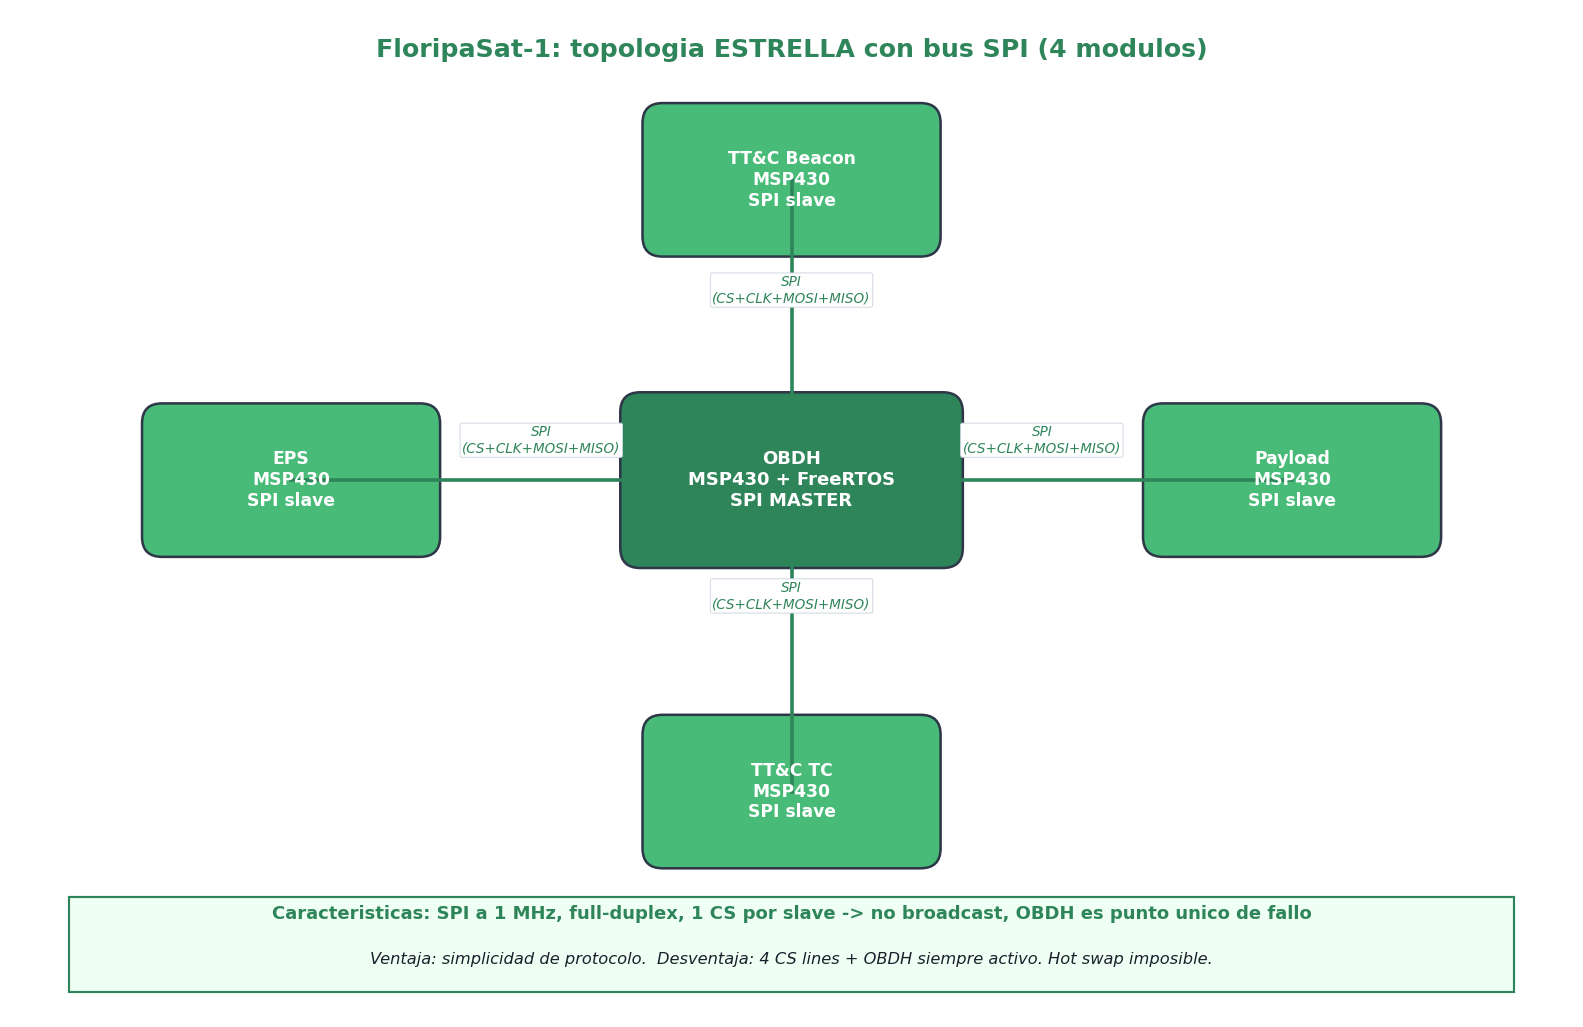
\includegraphics[width=\textwidth]{fig04_floripasat.png}
  \caption{Topologia de FloripaSat-1: estrella SPI alrededor del OBDH.
  Cada perif. es un MSP430 independiente con su firmware.}
  \label{fig:m15-floripasat}
\end{figure}

\section{El diseno}

\textbf{Cuatro modulos perifericos} (EPS, Payload, Beacon TT\&C,
Telecomando TT\&C) conectados al OBDH por SPI. Cada modulo es un
MSP430 con FreeRTOS propio.

\textbf{Senales SPI:} CLK, MOSI, MISO compartidas. Una linea CS por
slave (4 CS lines en total).

\textbf{Master:} siempre el OBDH. Los esclavos no pueden iniciar
transferencias: hay que esperar a que el OBDH les pregunte.

\section{Por que SPI y no I2C}

UFSC eligio SPI por:
\begin{enumerate}[leftmargin=2em]
  \item \textbf{Throughput}: SPI a 1 MHz es 2.5x mas rapido que I2C
    a 400 kHz, y full-duplex.
  \item \textbf{Inmunidad a fallas en un slave}: en I2C, un slave
    mal hecho puede colgar el bus entero (clock stretching infinito).
    En SPI no.
  \item \textbf{Determinismo}: en SPI el master controla todo el
    timing. No hay arbitraje.
\end{enumerate}

\section{Control}

\textbf{100\% centralizado}: el OBDH corre la FSM global, lee
telemetria de cada slave en un loop y emite comandos cuando hay que
cambiar de modo. Los slaves no toman decisiones --- solo responden.

\section{Lo que no funciona}

\begin{cuidado}
\textbf{Si el OBDH se cuelga, el satelite muere.} No hay forma de que
los slaves hablen entre si o con tierra sin pasar por el OBDH. UFSC
mitigo esto con un watchdog hardware externo que resetea el OBDH si
no se reporta cada N segundos.

Tampoco hay hot swap: si conectas/desconectas un slave en orbita
(imposible, pero conceptualmente), el bus SPI se rompe porque las
lineas CLK/MOSI quedan flotando.
\end{cuidado}

% ============================================================================
\chapter{OreSat: bus CAN multidrop con CANopen}
% ============================================================================

\begin{figure}[h]
  \centering
  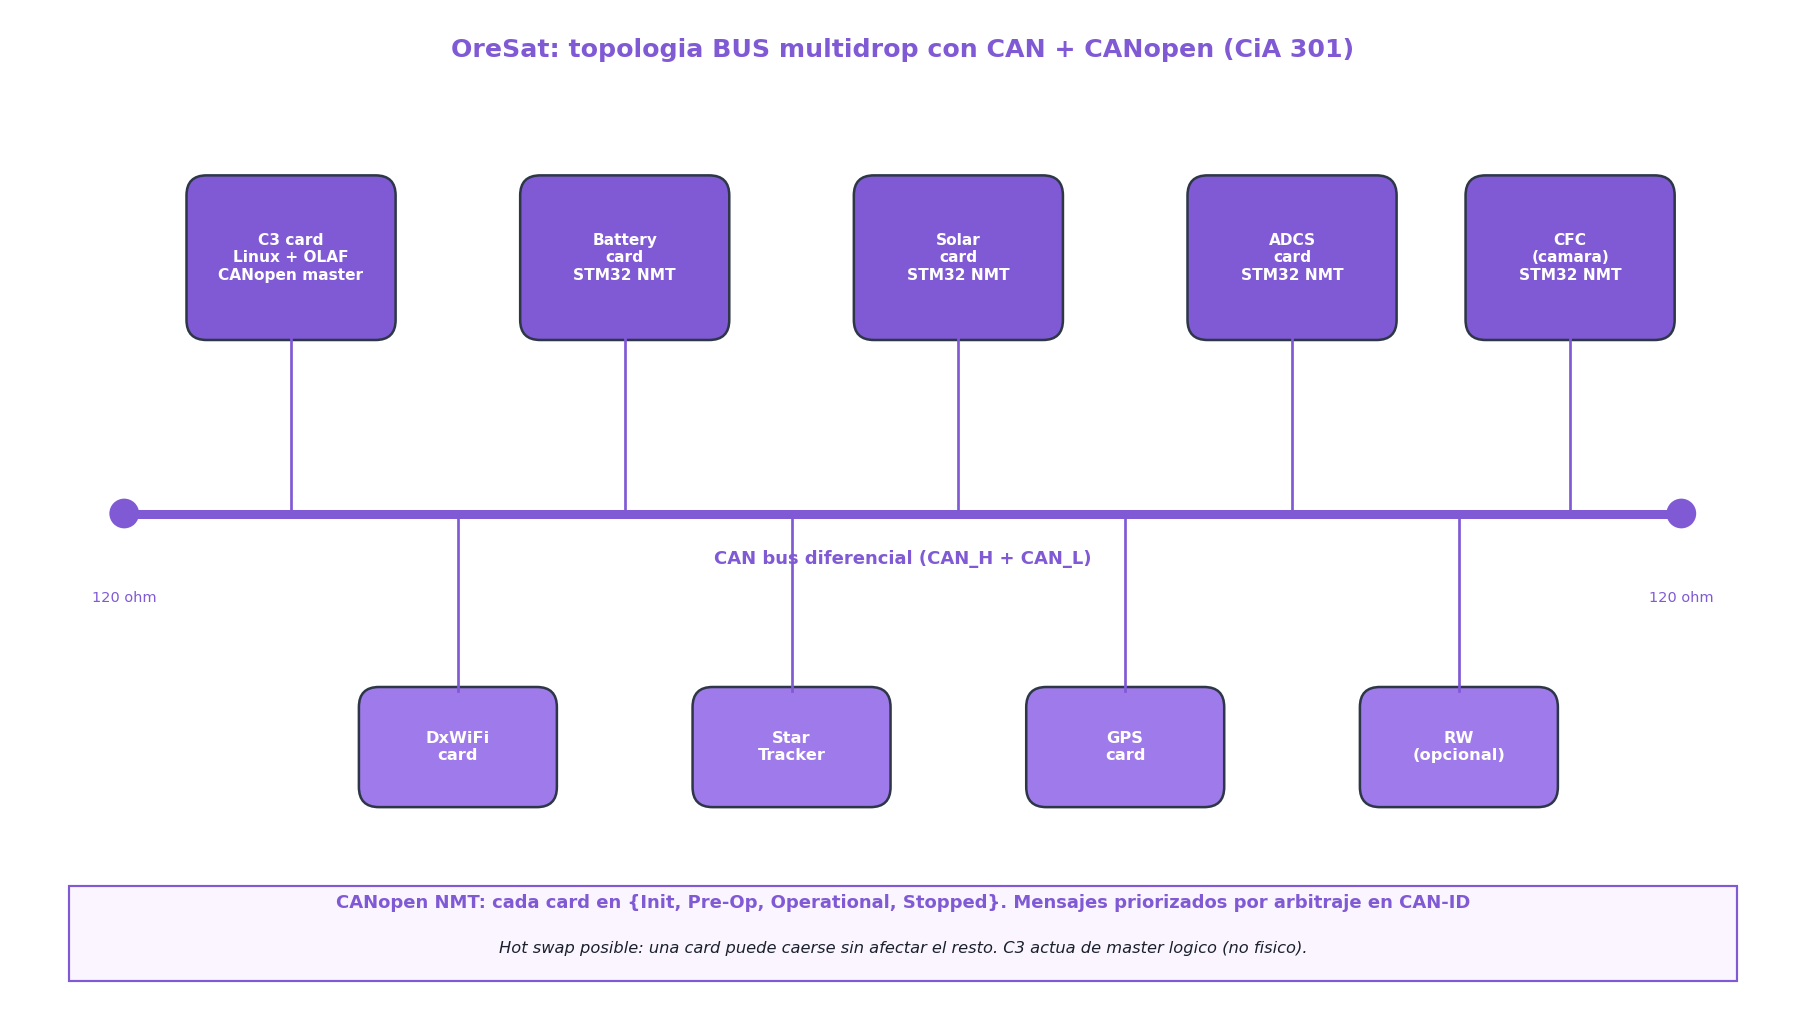
\includegraphics[width=\textwidth]{fig05_oresat.png}
  \caption{OreSat: bus CAN linear con terminadores de 120 ohm y cards
  CANopen. La C3 actua como master logico, no como master fisico.}
  \label{fig:m15-oresat}
\end{figure}

\section{El diseno}

\textbf{Un solo par diferencial} CAN\_H + CAN\_L recorre el cubesat de
punta a punta, con terminadores de 120 ohm en cada extremo. Todas las
\emph{cards} (subsistemas) cuelgan de este bus.

\textbf{Cada card es un STM32} con un transceiver CAN (TJA1042 tipico)
y un perfil CANopen. La excepcion es la \textbf{C3 card}, que corre
Linux con un demonio Python (OLAF) y actua de master logico.

\section{Por que CAN}

OreSat lo eligio por tres razones:

\begin{enumerate}[leftmargin=2em]
  \item \textbf{Robustez electrica}: senal diferencial, inmune a
    ruido. CAN nacio para autos en condiciones agresivas.
  \item \textbf{Multi-master}: cualquier card puede transmitir cuando
    necesita. El arbitraje por ID resuelve colisiones sin perder
    paquetes.
  \item \textbf{Estandar abierto}: CANopen CiA 301 es publico. Object
    Dictionary uniforme entre cards.
\end{enumerate}

\section{Control con CANopen}

\textbf{Distribuido pero coordinado.} Cada card tiene su FSM NMT
estandar (Init -> Pre-Op -> Operational -> Stopped). La C3 manda
mensajes NMT para forzar transiciones globales (``todos a
Pre-Operational''), pero cada card mantiene su propia logica interna.

\begin{tecnico}
\textbf{PDO vs SDO en CANopen.}
\begin{itemize}[leftmargin=2em]
  \item \textbf{PDO (Process Data Object)}: telemetria periodica
    publicada por la card sin pedido. Cada card publica sus PDOs en
    sus IDs reservados. Bajo overhead, ideal para housekeeping.
  \item \textbf{SDO (Service Data Object)}: lectura/escritura
    sincrona pedida por otro nodo (tipicamente la C3). Mayor overhead
    pero confiable.
\end{itemize}
\end{tecnico}

\section{Lo bueno y lo malo}

\textbf{Bueno:} si una card falla, el bus sigue (terminadores y
transceivers la aislan electricamente). Hot swap fisico es teoricamente
posible. La C3 puede inicializar el satelite sin saber a priori que
cards estan conectadas (NMT \emph{discovery}).

\textbf{Malo:} mas hardware (transceiver en cada card), mas software
(stack CANopen), mas masa, mas BOM. Para un 1U universitario es muchas
veces over-engineered.

% ============================================================================
\chapter{AAUSAT: estrella I2C + CSP encima}
% ============================================================================

\begin{figure}[h]
  \centering
  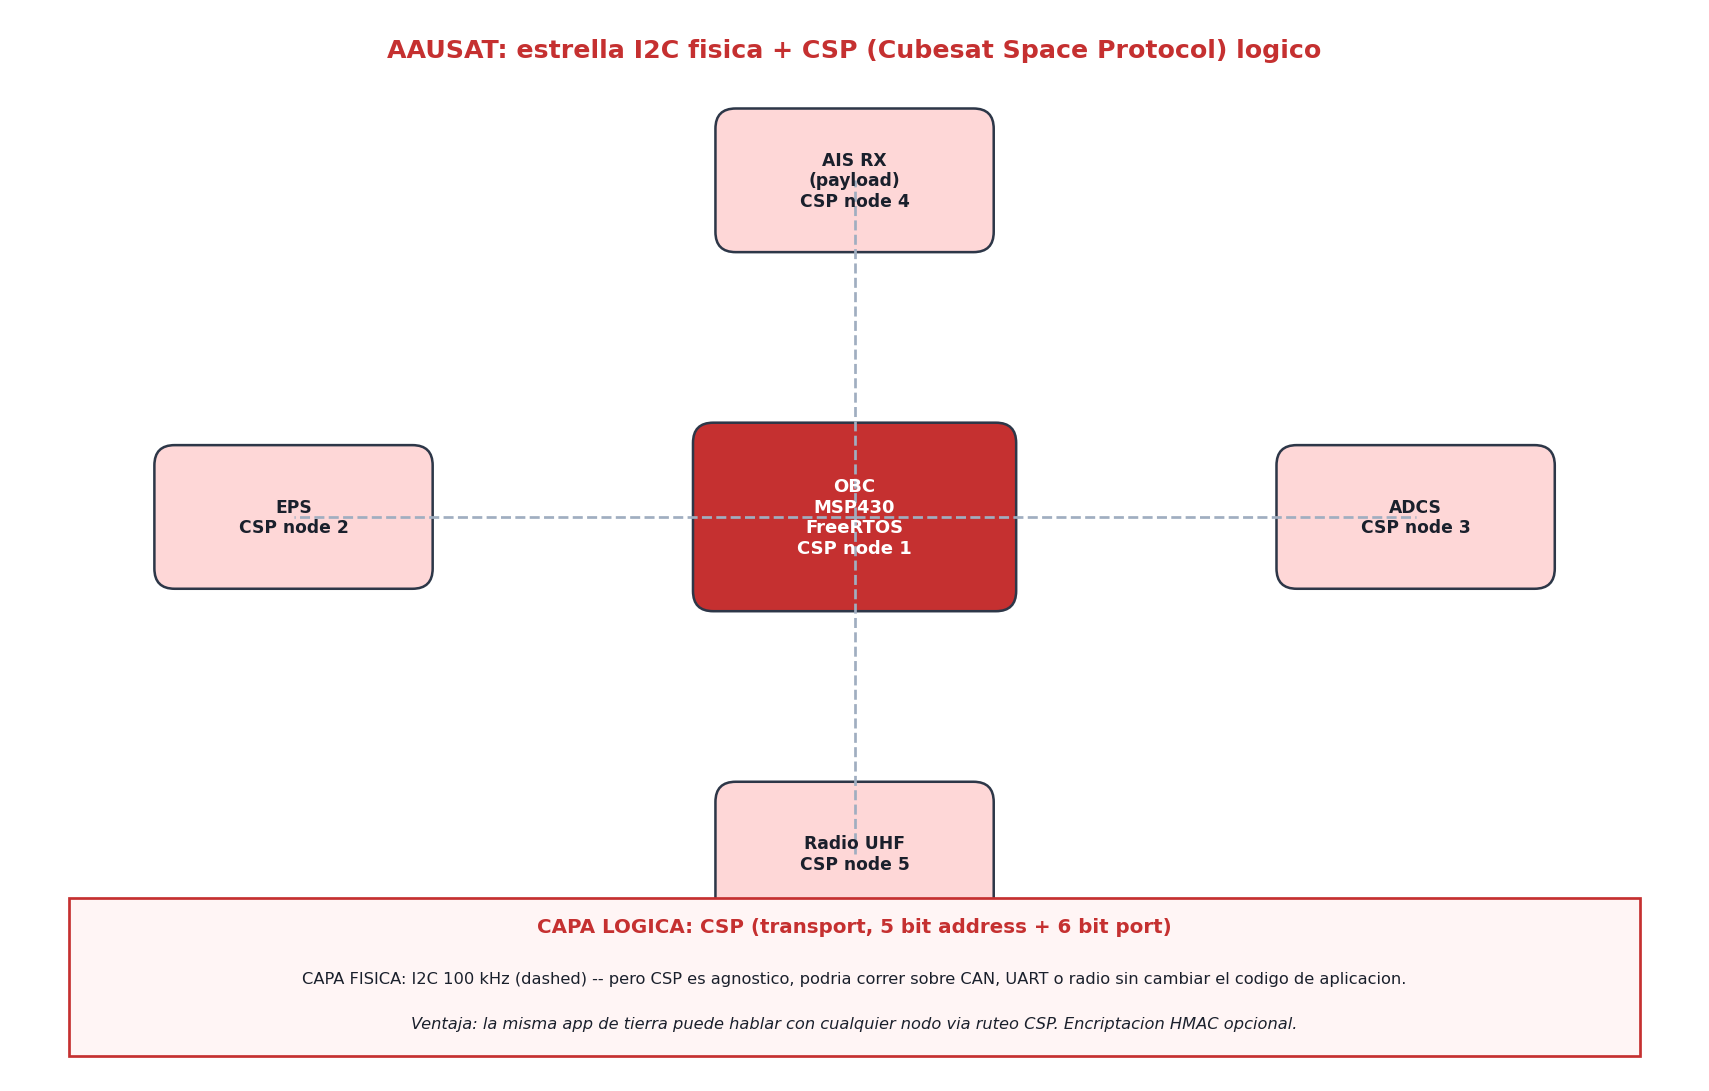
\includegraphics[width=\textwidth]{fig06_aausat.png}
  \caption{AAUSAT: capa fisica estrella I2C (lineas dashed) + capa
  logica CSP overlay. El codigo de aplicacion habla CSP, no I2C.}
  \label{fig:m15-aausat}
\end{figure}

\section{El diseno}

\textbf{Capa fisica:} estrella I2C, OBC al centro. Misma que UPSat.

\textbf{Capa logica:} \textbf{CSP (Cubesat Space Protocol)}. Es la
contribucion grande de Aalborg a la comunidad CubeSat. CSP es un
protocolo de red estilo TCP/IP especifico para satelites:

\begin{itemize}[leftmargin=2em]
  \item \textbf{Direcciones} de 5 bits (32 nodos posibles).
  \item \textbf{Puertos} de 6 bits (64 servicios por nodo).
  \item \textbf{Header} de 4 bytes con prioridad, source, destination,
    port y flags (HMAC, RDP, fragmentacion).
  \item \textbf{Capa agnostica del bus}: la misma app corre sobre
    I2C, CAN, UART o radio sin cambiar el codigo.
\end{itemize}

\section{Por que CSP fue revolucionario}

Antes de CSP, cada CubeSat reinventaba su protocolo de comandos. CSP
te permite escribir:

\begin{lstlisting}[style=c, caption=Envio de comando a otro nodo via CSP]
csp_packet_t * packet = csp_buffer_get(100);
strcpy((char *)packet->data, "GET_TLM");
packet->length = 7;

/* destino: nodo 2 (EPS), puerto 10 (telemetria) */
csp_send(conn, packet, /* timeout */ 1000);
\end{lstlisting}

\textbf{Y eso funciona igual} si el EPS esta colgado de I2C, de CAN
o llegando por radio. La libreria \texttt{libcsp} (open source, MIT)
se encarga del ruteo.

\section{Control}

Centralizado en el OBC, pero con una diferencia importante: el OBC
no envia bytes a una direccion I2C, envia paquetes a un nodo logico.
Si manana el EPS deja de estar en I2C y pasa a estar accesible por
otro bus, el codigo de aplicacion del OBC \textbf{no cambia}.

\begin{logrado}
INTISAT podria adoptar libcsp en v2 sin cambiar la topologia fisica.
Quedaria estrella I2C como L1+L2, CSP como L3+L4. Pago: una
dependencia C portada a Python (existe wrapper). Gano: rigor de capa
de red y futuro-proof.
\end{logrado}

% ============================================================================
\chapter{UPSat: estrella I2C sin capa de red}
% ============================================================================

\begin{figure}[h]
  \centering
  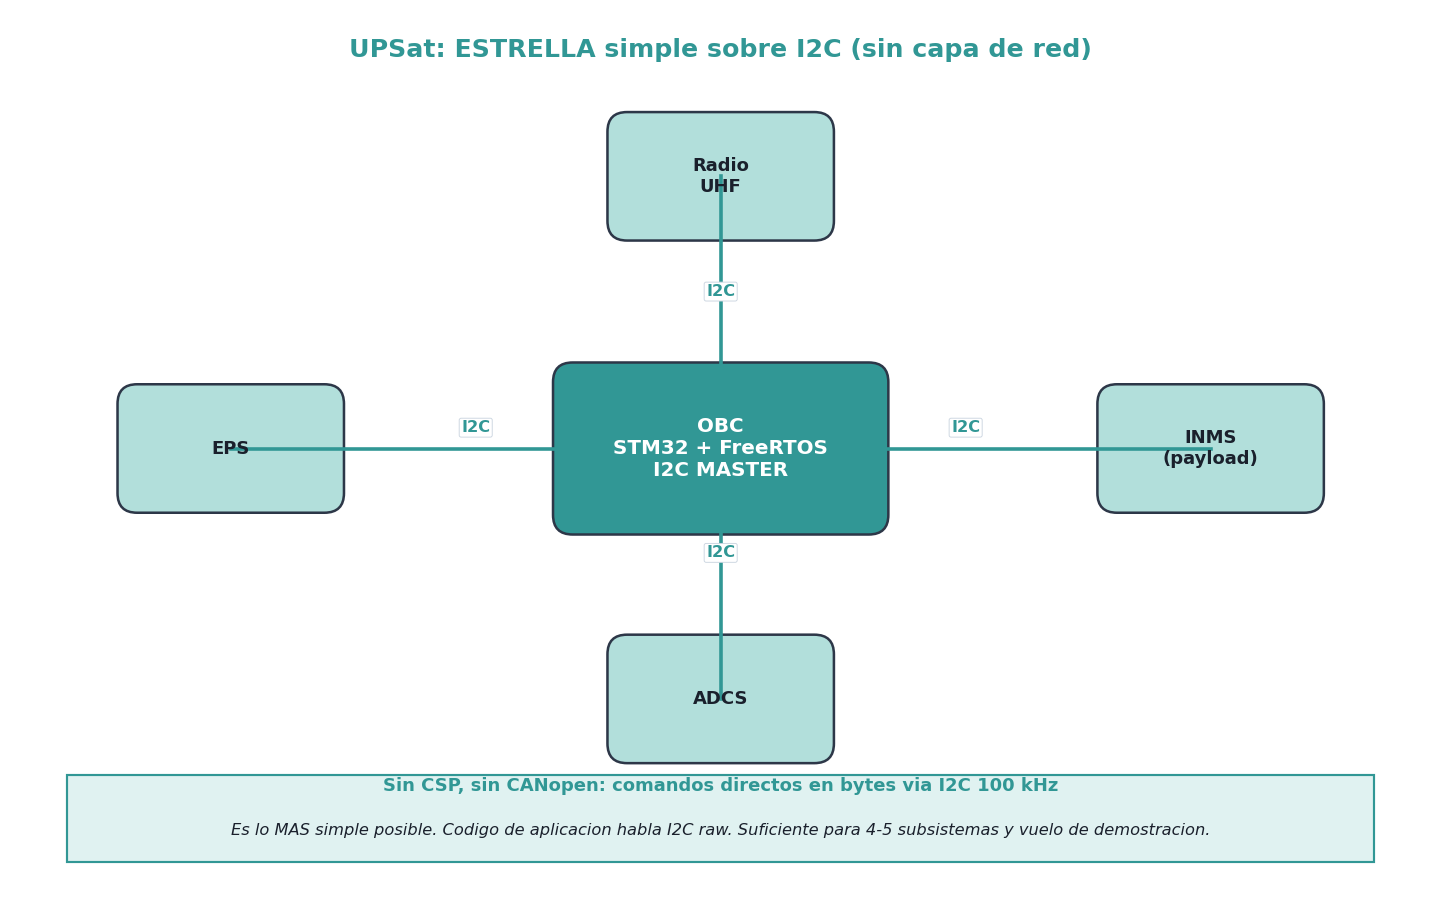
\includegraphics[width=0.9\textwidth]{fig07_upsat.png}
  \caption{UPSat: lo mas simple posible. Estrella I2C, sin CSP, sin
  CANopen. Comandos directos byte-a-byte.}
  \label{fig:m15-upsat}
\end{figure}

\section{El diseno}

\textbf{Estrella I2C}, OBC central, 4 perifericos (EPS, INMS payload,
radio UHF, ADCS). \textbf{Sin capa de red}: el codigo de aplicacion
escribe directamente en direcciones I2C.

\begin{lstlisting}[style=c, caption=Comando a un periferico en UPSat estilo]
uint8_t cmd[4] = { CMD_GET_TLM, 0x00, 0x00, 0x00 };
i2c_write(EPS_ADDR, cmd, 4);
i2c_read(EPS_ADDR, response_buffer, 16);
/* verificar CRC a mano */
\end{lstlisting}

\section{Por que funciona}

\textbf{Para 4 perifericos, una mision de demostracion y un equipo
chico, alcanza}. El stack de software es ~100 lineas de C por
periferico. No hay que aprender CSP ni CANopen. El tiempo de
desarrollo es 5x menor que cualquier alternativa con capa de red.

\section{Donde se rompe}

\begin{cuidado}
Si la mision crece (mas subsistemas, mas comandos, mas variantes),
el codigo de aplicacion empieza a ser un monstruo de \texttt{if/else}
sobre direcciones I2C. Cualquier cambio en el cableado fisico
obliga a reescribir el codigo de comandos.

UPSat duro 6 meses en orbita y fue suficiente. Para una mision de
2 anos o con un payload complejo (como INTISAT), probablemente
quieras CSP.
\end{cuidado}

% ============================================================================
\chapter{NASA cFS: Software Bus pub/sub}
% ============================================================================

\begin{figure}[h]
  \centering
  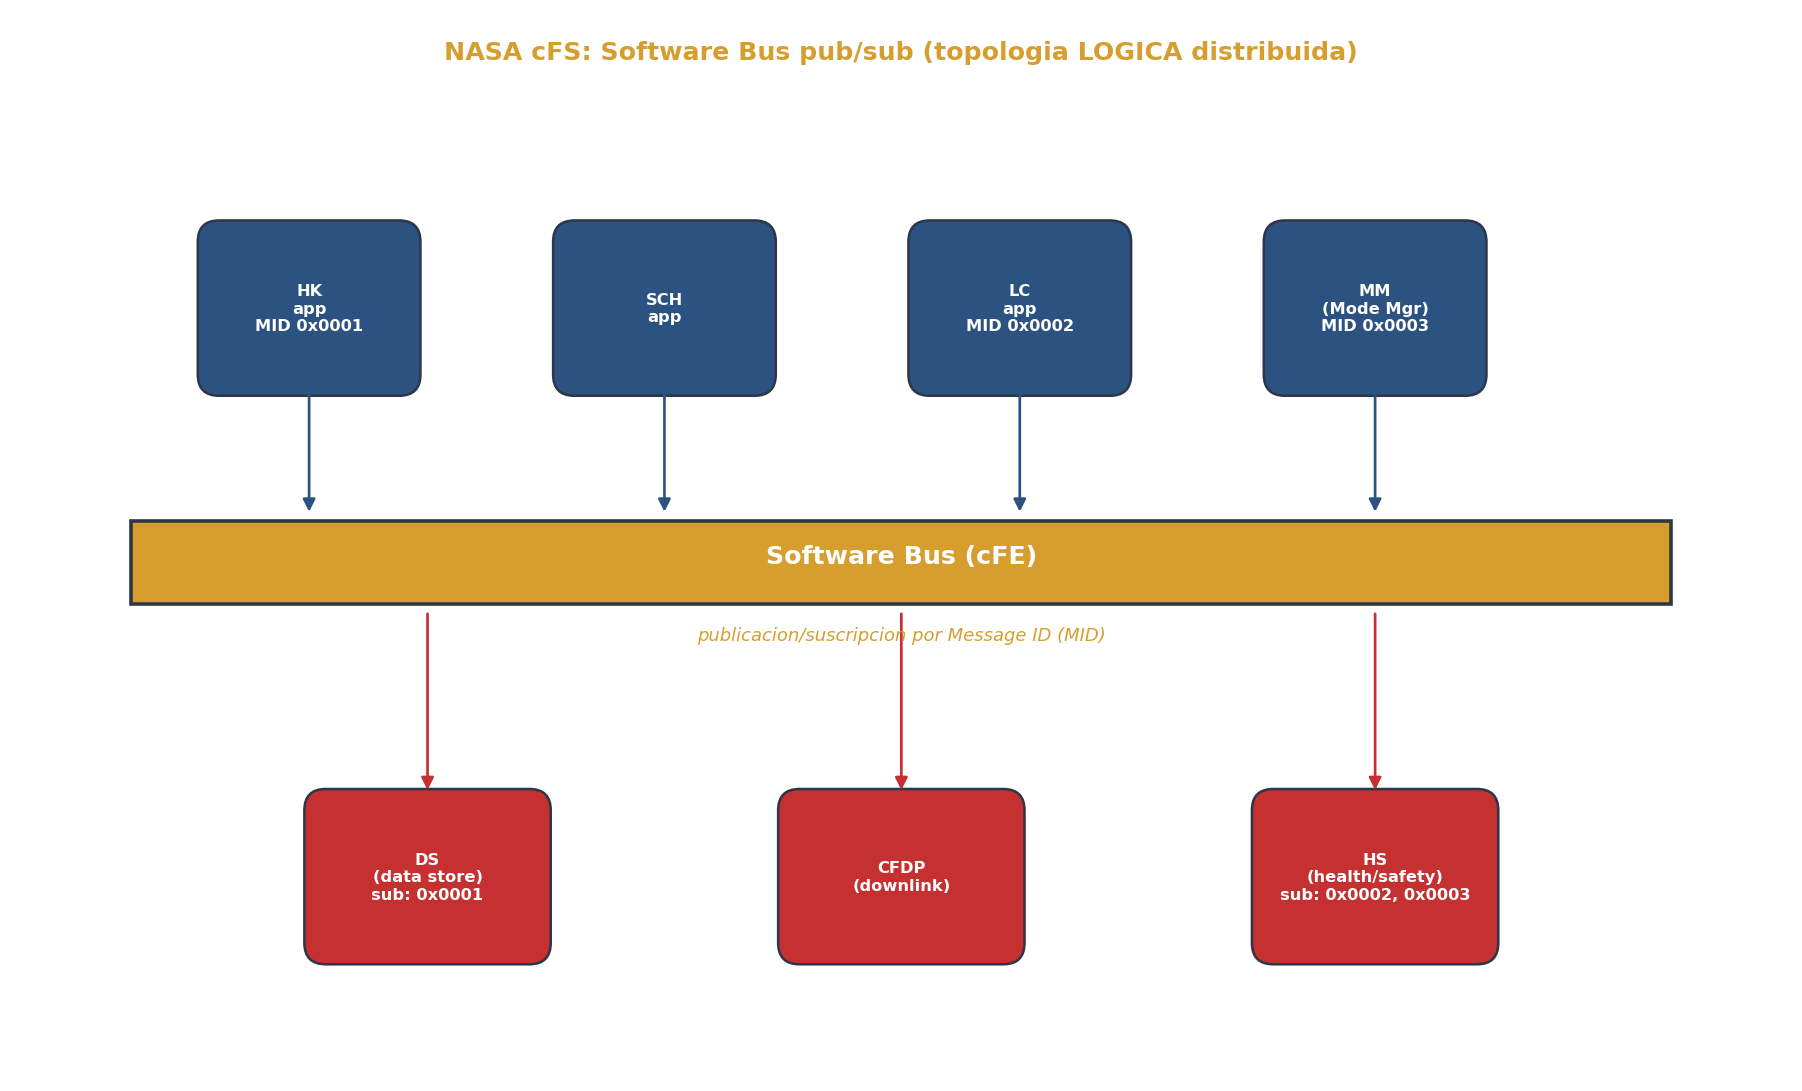
\includegraphics[width=\textwidth]{fig08_cfs.png}
  \caption{NASA cFS: las apps no se conocen entre si. Publican
  mensajes con un Message ID (MID) y otras apps se suscriben. El
  Software Bus es el central.}
  \label{fig:m15-cfs}
\end{figure}

\section{El diseno}

\textbf{No hay bus fisico definido por cFS.} Lo que define cFS es la
capa de software: un \emph{Software Bus} corriendo en el OBC al que
las apps publican mensajes por \emph{Message ID} (MID, 16 bits) y
otras apps se suscriben.

\textbf{Las apps no se conocen entre si.} La app HK publica un
mensaje de housekeeping. Las apps DS (Data Storage), CFDP (downlink),
HS (Health \& Safety) pueden suscribirse, cada una por sus razones,
sin que HK sepa quien escucha.

\section{Por que esto es topologia}

Aunque fisicamente todo corre en el mismo procesador, \textbf{la
topologia logica es distribuida}. Es la misma idea que ROS2 o que
DDS: separar el ``que publico'' del ``quien lee''.

\textbf{Cuando hay multiples procesadores} (Lunar IceCube, MMS), el
Software Bus se extiende sobre la red real (SpaceWire tipico). Pero
el codigo de las apps no se entera.

\section{Control}

\textbf{No hay un control central}, hay reglas. La app
\textbf{Mode Manager} publica el modo actual. Otras apps
\emph{reaccionan} (DS guarda menos datos en modo SAFE, etc).

\begin{intui}
La diferencia conceptual con FloripaSat o UPSat es enorme: en cFS,
nadie ``manda''. El estado del satelite es un \emph{shared truth}
publicado en el Software Bus. Esto reduce muchisimo el acoplamiento
pero requiere disciplina para que todas las apps sepan exactamente
en que MIDs publicar.
\end{intui}

% ============================================================================
\chapter{NASA F\textquotesingle{}: topologia compile-time}
% ============================================================================

\begin{figure}[h]
  \centering
  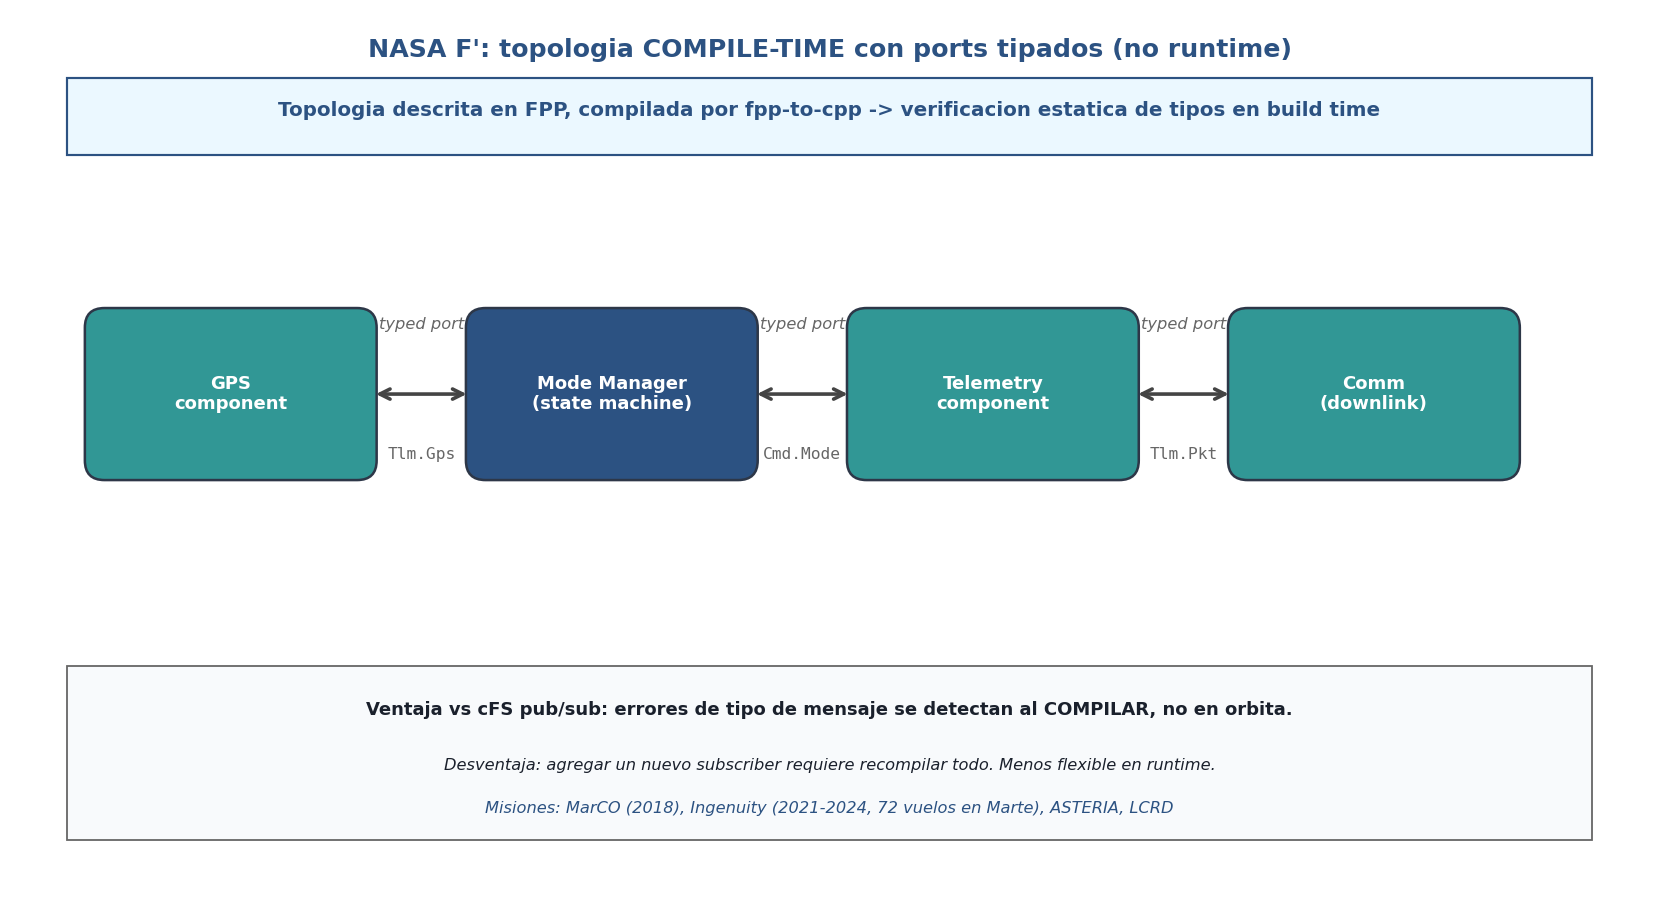
\includegraphics[width=\textwidth]{fig09_fprime.png}
  \caption{F\textquotesingle{}: la topologia se declara en FPP y se compila. No hay
  ``descubrimiento'' en runtime, todas las conexiones son estaticas
  y tipadas.}
  \label{fig:m15-fprime}
\end{figure}

\section{El diseno}

\textbf{Componentes conectados por ports tipados.} La topologia
completa esta en un archivo \texttt{.fpp} (F Prime Prime). Cuando
ejecutas \texttt{fpp-to-cpp}, el compilador genera el codigo de las
conexiones, verifica que los tipos coincidan, y produce C++.

\section{Por que esto es distinto de cFS}

\begin{itemize}[leftmargin=2em]
  \item \textbf{cFS (pub/sub):} agregar un suscriptor nuevo es trivial,
    se hace en runtime. Pero si publicas un MID que nadie escucha,
    nadie te avisa.
  \item \textbf{F\textquotesingle{} (compile-time):} si conectas dos ports
    incompatibles, no compila. Pero agregar un componente nuevo
    requiere recompilar todo.
\end{itemize}

\textbf{Trade-off claro:} flexibilidad runtime (cFS) vs verificacion
estatica (F\textquotesingle{}).

\section{Donde gano F\textquotesingle{}}

F\textquotesingle{} volo en MarCO (2018, primeros CubeSats a Marte), en Ingenuity (72
vuelos en Marte 2021-2024), en ASTERIA, en NEA Scout. Es el framework
que mas saco la NASA al espacio profundo en los ultimos 8 anos.

El argumento de JPL fue: \emph{a 5--20 minutos de retardo de senal,
queremos errores de tipo detectados en compilacion, no en orbita}.
Tiene sentido.

% ============================================================================
\chapter{Matriz comparativa}
% ============================================================================

\begin{figure}[h]
  \centering
  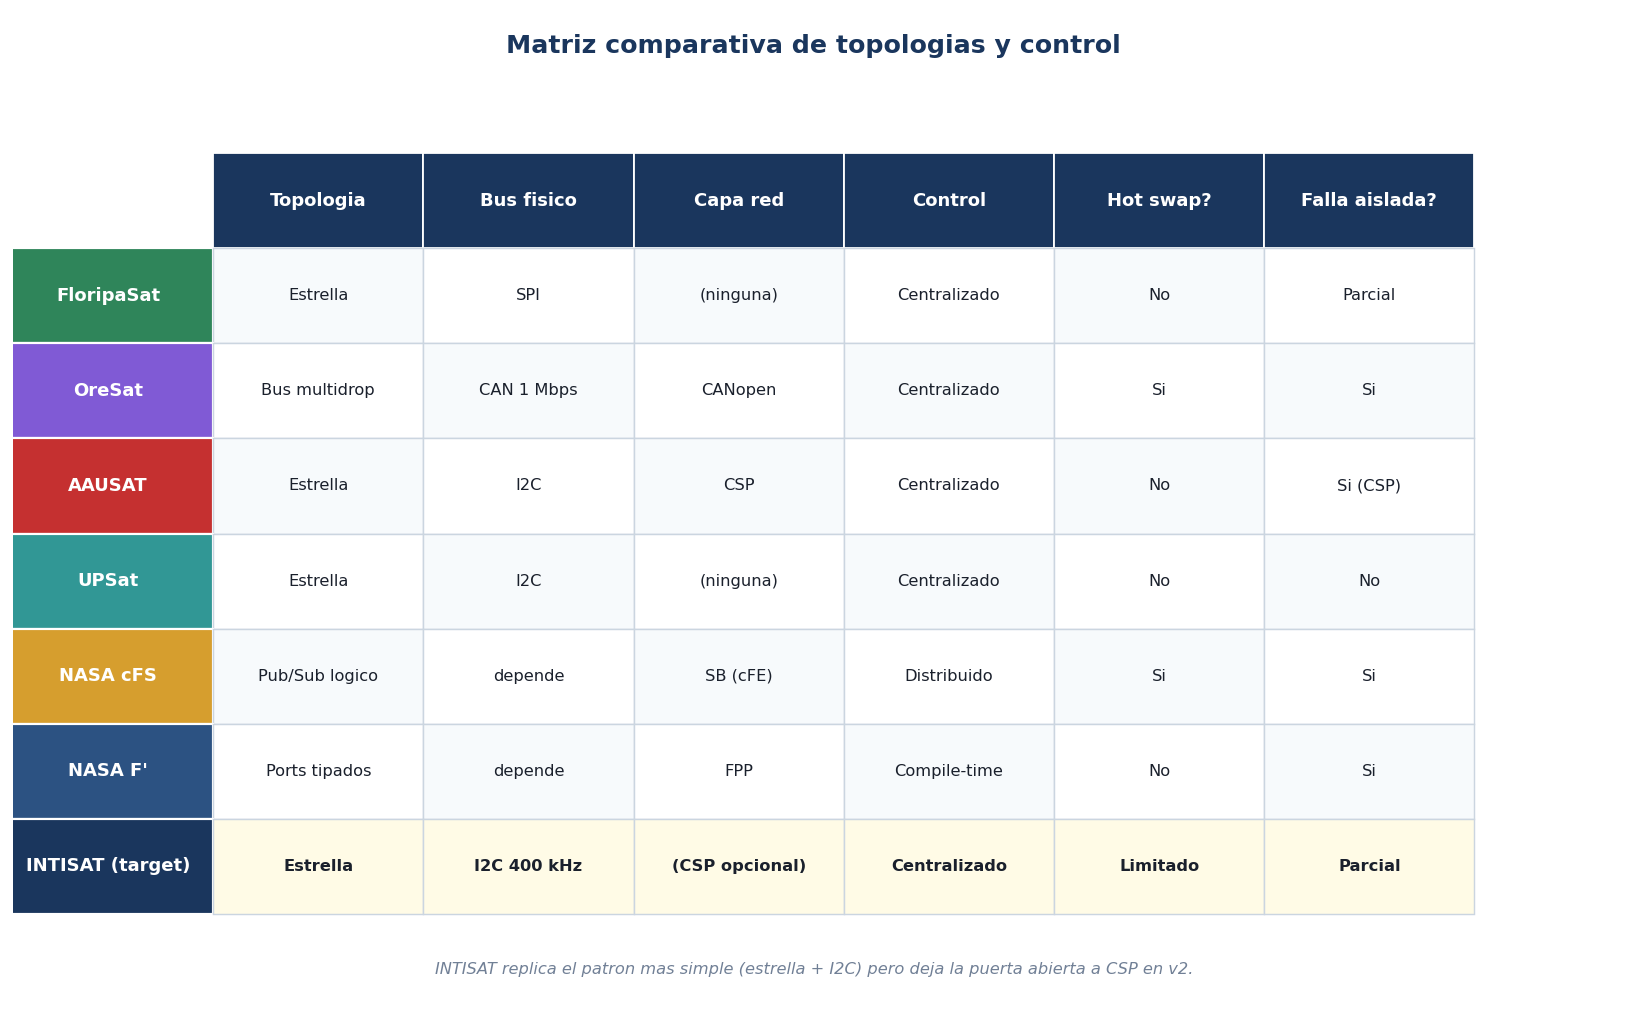
\includegraphics[width=\textwidth]{fig10_matriz.png}
  \caption{Matriz: las 6 misiones de referencia + INTISAT contra 6
  dimensiones (topologia, bus fisico, capa red, control, hot swap,
  aislamiento de falla).}
  \label{fig:m15-matriz}
\end{figure}

\section{Lectura de la matriz}

\textbf{Patrones que valen la pena marcar:}

\begin{enumerate}[leftmargin=2em]
  \item \textbf{Estrella + I2C} es el patron por defecto en CubeSats
    universitarios chicos. UPSat, AAUSAT, INTISAT. Lo mas simple que
    funciona.
  \item \textbf{Bus multidrop + CAN} aparece cuando hay mas de 5--6
    subsistemas y queres independencia. OreSat. GomSpace en sus
    modulos modernos.
  \item \textbf{Capa de red explicita} (CSP, CANopen, SB) es lo que
    diferencia un proyecto serio de uno de demostracion. UPSat no la
    tiene y se nota: cambiar cualquier cosa rompe todo.
  \item \textbf{Pub/sub} (cFS) y \textbf{compile-time} (F\textquotesingle{}) son
    aproximaciones \emph{profesionales}. Requieren equipos con
    experiencia.
\end{enumerate}

\section{La decision de INTISAT en contexto}

INTISAT replica el patron mas simple: estrella + I2C, sin capa de red
en la primera version. Es una decision \emph{deliberada}:

\begin{itemize}[leftmargin=2em]
  \item Sabemos que es lo mas conservador.
  \item Sabemos que pierde futuro-proof.
  \item Pero el equipo tiene experiencia con I2C y \emph{cero}
    experiencia con CSP/CANopen.
\end{itemize}

\textbf{La trampa a evitar} es decir ``mejor ya empezamos con CAN +
CANopen porque es mas profesional''. Eso aumenta el riesgo de cronograma
sin beneficio claro para una mision de demostracion 1U.

% ============================================================================
\chapter{Como se ejerce el control}
% ============================================================================

\section{Los 4 modelos de control}

\begin{enumerate}[leftmargin=2em]
  \item \textbf{Centralizado puro.} OBC manda comandos, los perifericos
    obedecen. FloripaSat, UPSat. Simple, riesgo de single-point-of-failure.
  \item \textbf{Centralizado con autonomia local.} El OBC manda en
    grande, cada periferico tiene su FSM interna para emergencias.
    AAUSAT con CSP. INTISAT propuesto.
  \item \textbf{Distribuido coordinado.} Cada subsistema tiene su
    propia FSM pero todos siguen un \emph{shared truth}. OreSat con NMT,
    NASA cFS con Mode Manager.
  \item \textbf{Compile-time.} La topologia y las conexiones se fijan
    al compilar. No hay descubrimiento. F\textquotesingle{}.
\end{enumerate}

\section{Flujo temporal de un comando}

Para hacer concreto el control, veamos como viaja un telecomando desde
tierra hasta el subsistema que tiene que ejecutarlo.

\begin{figure}[h]
  \centering
  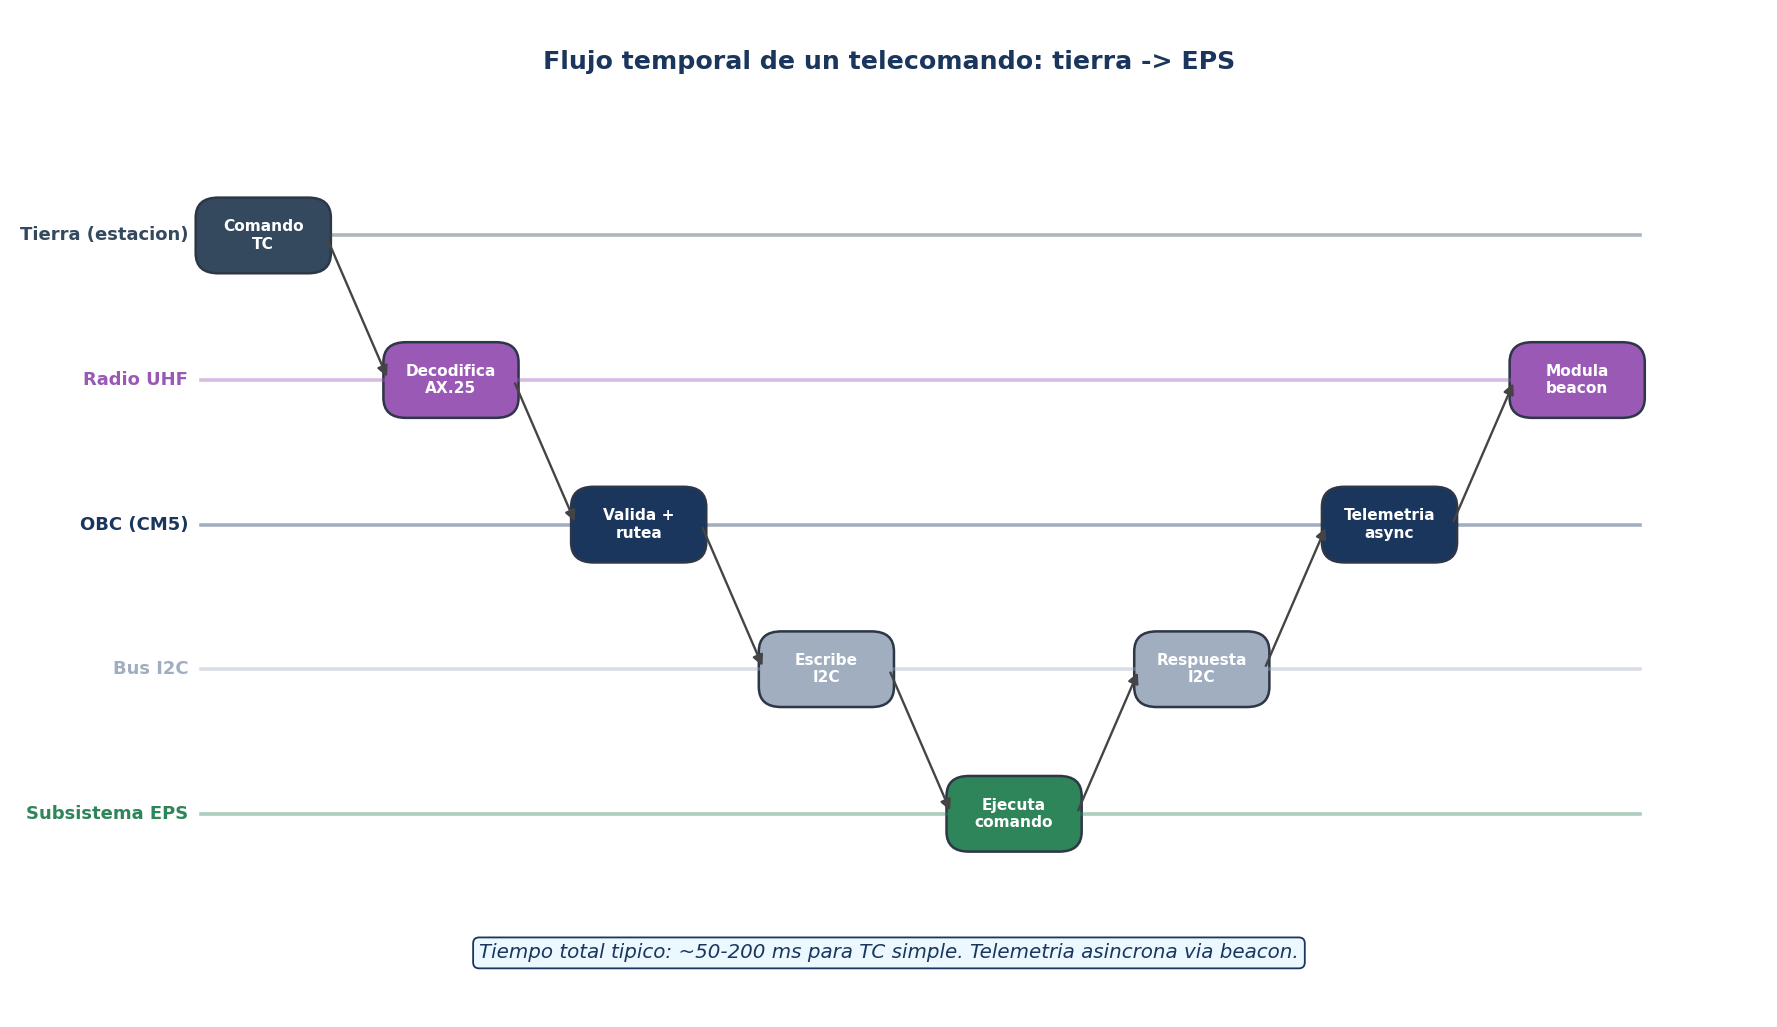
\includegraphics[width=\textwidth]{fig12_flujo_control.png}
  \caption{Flujo temporal: TC desde tierra hasta ejecucion en EPS,
  con respuesta asincrona via beacon. Tiempo total tipico
  50--200 ms.}
  \label{fig:m15-flujo}
\end{figure}

\textbf{Los pasos:}

\begin{enumerate}[leftmargin=2em]
  \item \textbf{Tierra} envia un paquete TC modulado en UHF.
  \item \textbf{Radio} demodula, decodifica el frame AX.25.
  \item \textbf{OBC} valida el comando (CRC, autenticacion) y decide
    a que subsistema redirigirlo.
  \item \textbf{Bus I2C}: el OBC escribe el comando en la direccion
    del EPS.
  \item \textbf{EPS} ejecuta. Suele ser inmediato (ms).
  \item \textbf{Respuesta I2C}: el EPS escribe un ACK + status.
  \item \textbf{Telemetria asincrona}: el OBC compone un paquete TM
    y lo encola.
  \item \textbf{Beacon UHF} retransmite la TM en el siguiente ciclo.
\end{enumerate}

\textbf{Tiempo total tipico:} 50--200 ms desde TC valido hasta accion
en HW. La respuesta de TM puede ser inmediata o esperar al proximo
beacon (cada N segundos).

\begin{tecnico}
\textbf{Por que la TM es asincrona.} Si el TC dispara una accion larga
(captura FPM = 180 s), no podemos bloquear el beacon esperando. El
OBC encola la TM y la manda cuando hay tiempo de aire. Esto se aleja
del modelo request-response sincrono de HTTP, es mas parecido a un
sistema de eventos.
\end{tecnico}

% ============================================================================
\chapter{Propuesta de topologia para INTISAT}
% ============================================================================

\section{Decision: estrella I2C centrada en CM5}

\begin{figure}[h]
  \centering
  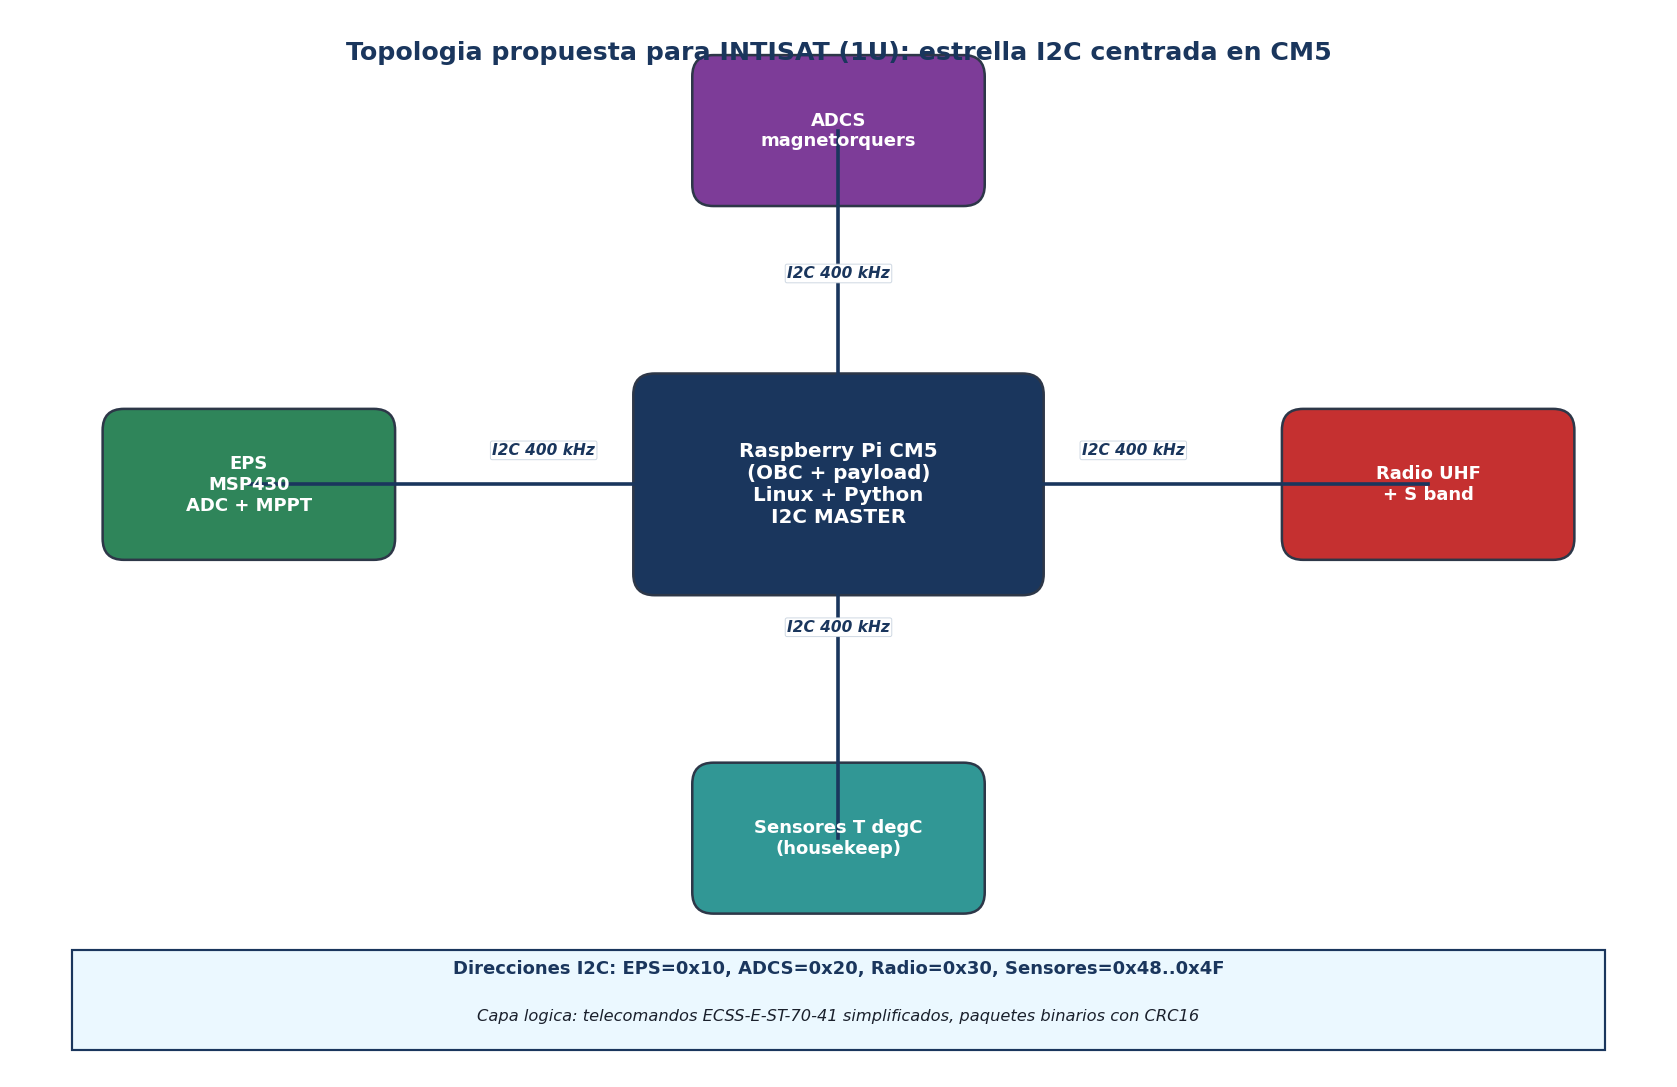
\includegraphics[width=\textwidth]{fig11_intisat.png}
  \caption{Topologia propuesta para INTISAT 1U: CM5 al centro como
  I2C master, 4 subsistemas perifericos.}
  \label{fig:m15-intisat}
\end{figure}

\textbf{Componentes:}

\begin{itemize}[leftmargin=2em]
  \item \textbf{CM5 (master)}: Raspberry Pi Compute Module 5, Linux
    + Python. OBC + payload integrados en el mismo SoC.
  \item \textbf{EPS}: MSP430 o STM32, en direccion I2C 0x10. Reporta
    SOC, voltajes de baterias, corrientes de paneles, temperatura.
  \item \textbf{ADCS}: STM32 con magnetorquers, en 0x20. Reporta
    orientacion estimada por magnetometro.
  \item \textbf{Radio UHF + S}: modulo comercial (EnduroSat o
    similar), en 0x30. Telemetria/telecomando + downlink payload.
  \item \textbf{Sensores T degC}: TMP117 en cadena, en 0x48..0x4F.
\end{itemize}

\section{Velocidad y eleccion electrica}

\textbf{I2C a 400 kHz} (Fast-mode). Suficiente para todos los
comandos previstos y los chunks de telemetria (<1 kB por comando).
No vamos a 1 MHz Fast-mode+ por riesgo de glitches con cables de
$\sim$15 cm dentro del 1U.

\textbf{Pull-ups: 4.7 kohm} en SDA y SCL. Estandar Fast-mode con
varios dispositivos.

\textbf{Logica 3.3 V} en todo el bus. CM5 ya es 3.3V. Hay que
verificar que el EPS lo sea (si es de 5V, level-shifter
bidireccional).

\section{Capa de aplicacion: paquetes binarios + CRC16}

Sin CSP en v1. Comandos como:

\begin{lstlisting}[style=py, caption=Estructura de telecomando hacia EPS]
# Header: [CMD_ID:1][PAYLOAD_LEN:1][PAYLOAD:N][CRC16:2]
def build_tc(cmd_id, payload):
    pkt = bytes([cmd_id, len(payload)]) + payload
    crc = crc16_ccitt(pkt)
    return pkt + crc.to_bytes(2, 'big')

def send_tc(eps_addr, cmd_id, payload=b''):
    pkt = build_tc(cmd_id, payload)
    with smbus2.SMBus(1) as bus:
        bus.write_i2c_block_data(eps_addr, 0, list(pkt))
\end{lstlisting}

\section{Roadmap}

\begin{logrado}
\textbf{v1 (mision de demostracion):} estrella I2C + paquetes binarios
con CRC16. Sin CSP, sin CANopen. Lo minimo que vuela.

\textbf{v2 (si hay segunda iteracion):} agregar \texttt{libcsp}
Python sobre el mismo I2C. Ganamos: direccionamiento logico,
fragmentacion, retries automaticos. Costo: $\sim$2 semanas de
desarrollo + tests.

\textbf{Lo que NO vamos a hacer:} pasar a CAN. Para 4 perifericos no
se justifica el costo de transceivers + stack CANopen, sobre todo
sin experiencia previa del equipo.
\end{logrado}

\section{Lo que tenemos que decidir aun}

\begin{enumerate}[leftmargin=2em]
  \item \textbf{Direcciones I2C definitivas} por subsistema (propuesto
    arriba pero falta confirmar con EPS comercial elegido).
  \item \textbf{Formato exacto del header de paquete} (32 bits? 64
    bits? compatible con ECSS?)
  \item \textbf{Politica de retries}: cuantos antes de declarar
    error?
  \item \textbf{Diagnostico de bus}: tenemos que poder leer SCL y SDA
    desde la CM5 (analizador logico via GPIO) para debugging?
\end{enumerate}

\appendix

\chapter{Glosario}

\begin{description}[leftmargin=4em, style=nextline]
  \item[ACK] Acknowledge, paquete de confirmacion.
  \item[AX.25] Protocolo de capa enlace usado en radio amateur.
  \item[CAN] Controller Area Network. Bus serial diferencial.
  \item[CANopen] Perfil de aplicacion estandar sobre CAN (CiA 301).
  \item[CCSDS] Consultative Committee for Space Data Systems.
  \item[cFE] Core Flight Executive. Runtime de NASA cFS.
  \item[CRC] Cyclic Redundancy Check. Codigo de deteccion de errores.
  \item[CS] Chip Select. Linea de seleccion de esclavo en SPI.
  \item[CSP] Cubesat Space Protocol. Capa de red para CubeSats.
  \item[DDS] Data Distribution Service. Middleware pub/sub.
  \item[ECSS] European Cooperation for Space Standardization.
  \item[FPP] F Prime Prime. DSL textual de NASA F\textquotesingle{}.
  \item[Frame] Unidad de datos en capa enlace.
  \item[Hot swap] Conectar/desconectar dispositivos sin apagar.
  \item[I2C] Inter-Integrated Circuit. Bus serial 2-hilos.
  \item[MAC] Medium Access Control. Subcapa de enlace.
  \item[MID] Message ID. Identificador de mensaje en cFS Software Bus.
  \item[Multidrop] Topologia donde varios nodos comparten el mismo bus
    fisico.
  \item[NMT] Network Management. Servicio CANopen.
  \item[OBC] On-Board Computer.
  \item[OBDH] On-Board Data Handling. Equivalente OBC.
  \item[OSI] Open Systems Interconnection. Modelo de capas de red.
  \item[PDO] Process Data Object. Telemetria periodica en CANopen.
  \item[RS-232 / RS-485] Estandares electricos serial.
  \item[SB] Software Bus de cFS.
  \item[SDO] Service Data Object. Lectura sincrona en CANopen.
  \item[SOC] State of Charge (bateria).
  \item[SpaceWire] Estandar ECSS-E-ST-50-12C. Bus alta velocidad para
    misiones grandes.
  \item[SPI] Serial Peripheral Interface. Bus serial 4-hilos.
  \item[Star / Estrella] Topologia con hub central.
  \item[TC / TM] Telecomando / Telemetria.
  \item[Transceiver] Chip que convierte logica a senal diferencial.
  \item[UART] Universal Asynchronous Receiver Transmitter.
\end{description}

\chapter{Referencias y URLs verificables}

\section{Estandares}

\begin{itemize}[leftmargin=2em]
  \item I2C spec (NXP / Philips): \url{https://www.nxp.com/docs/en/user-guide/UM10204.pdf}
  \item CAN spec (Bosch): \url{https://www.bosch-semiconductors.com/}
  \item CANopen CiA 301: \url{https://www.can-cia.org/can-knowledge/canopen/}
  \item SpaceWire ECSS-E-ST-50-12C: \url{https://ecss.nl/}
  \item AX.25 (radio amateur): TAPR documentacion publica.
  \item CCSDS Packet Telemetry: \url{https://public.ccsds.org/Publications/BlueBooks.aspx}
\end{itemize}

\section{Protocolos open source para CubeSats}

\begin{itemize}[leftmargin=2em]
  \item \textbf{libcsp} (AAUSAT origen): \url{https://github.com/libcsp/libcsp}
  \item \textbf{python-csp}: implementaciones varias en Python.
  \item \textbf{CANopenNode}: \url{https://github.com/CANopenNode/CANopenNode}
\end{itemize}

\section{Frameworks NASA}

\begin{itemize}[leftmargin=2em]
  \item NASA cFS: \url{https://github.com/nasa/cFS}
  \item NASA F\textquotesingle{}: \url{https://github.com/nasa/fprime}
  \item FPP language: \url{https://nasa.github.io/fpp/}
\end{itemize}

\section{Repos de las misiones}

\begin{itemize}[leftmargin=2em]
  \item FloripaSat (UFSC): \url{https://github.com/floripasat}
  \item OreSat (PSU): \url{https://github.com/oresat}
  \item UPSat (Libre Space): \url{https://gitlab.com/librespacefoundation/upsat/}
  \item AAUSAT: \url{https://www.space.aau.dk/cubesat/}
\end{itemize}

\section{Material de lectura recomendado}

\begin{itemize}[leftmargin=2em]
  \item NASA cFS tutorial (Goddard, YouTube): introduce todo el stack
    en $\sim$2 horas.
  \item NASA F\textquotesingle{} Hello World: \url{https://nasa.github.io/fprime/Tutorials/HelloWorld/Tutorial.html}
  \item ``CubeSat Communication System, a New Open Source Design''
    --- Aalborg paper sobre CSP.
\end{itemize}

\end{document}
